\documentclass[serif,9pt]{beamer}
\usetheme{tree}

\usepackage[latin1]{inputenc}
\usepackage[spanish]{babel}
\usepackage{caption}
\usepackage{graphicx} % figuras
\usepackage{subfigure} % subfiguras
\usepackage{float}

\restylefloat{figure}

\beamersetuncovermixins{\opaqueness<1>{25}}{\opaqueness<2->{15}}

\begin{document}

\title{Pr�ctica 1: An�lisis de la eficiencia de algoritmos}  
\author{David Cabezas Berrido}
\date{}

\begin{frame}
\titlepage
\end{frame}

\begin{frame}\frametitle{Contenido}
\tableofcontents
\end{frame} 

\section{Eficiencia Emp�rica} 

\subsection{Algoritmos de orden de eficiencia $O(n^2)$}

\begin{frame}\frametitle{Algoritmos de orden de eficiencia $O(n^2)$} 

\begin{figure}[H]
  \centering
  \subfigure{\label{graf:n2}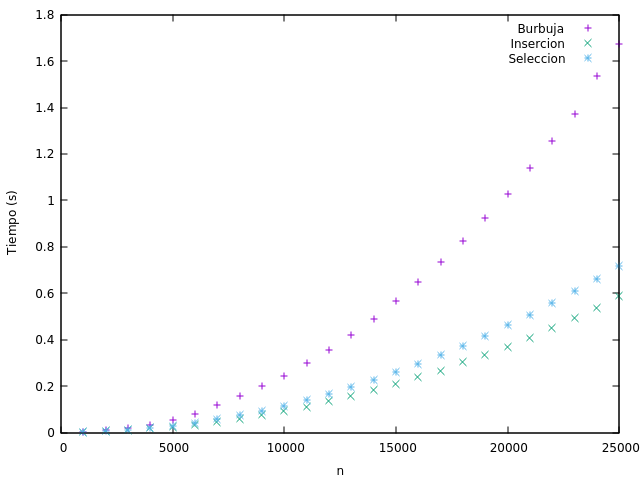
\includegraphics[width=95mm]{graficos/on2}}
\end{figure}

\end{frame}

\subsection{Algoritmos de orden de eficiencia $O(n\log n)$}
\begin{frame}\frametitle{Algoritmos de orden de eficiencia $O(n\log n)$}

  \begin{figure}[H]
    \centering
    \subfigure{\label{graf:nlogn}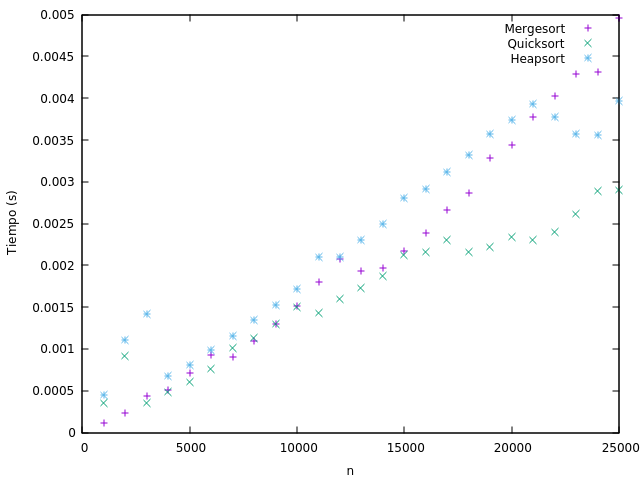
\includegraphics[width=95mm]{graficos/onlogn}}
    \end{figure}
  
  \end{frame}

\subsection{Algoritmos de orden de eficiencia $O(n^3)$}
\begin{frame}\frametitle{Algoritmos de orden de eficiencia $O(n^3)$}

  \begin{figure}[H]
    \centering
    \subfigure{\label{graf:n3}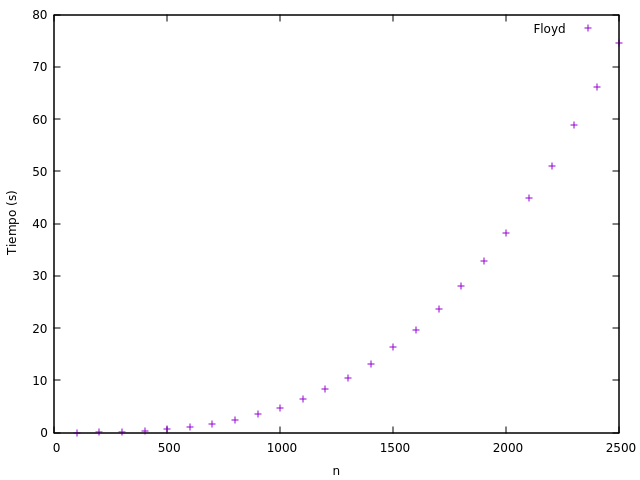
\includegraphics[width=95mm]{graficos/on3}}
    \end{figure}
  
  \end{frame}

\subsection{Algoritmos de orden de eficiencia $O(2^n)$}
\begin{frame}\frametitle{Algoritmos de orden de eficiencia $O(2^n)$}

  \begin{figure}[H]
    \centering
    \subfigure{\label{graf:2n}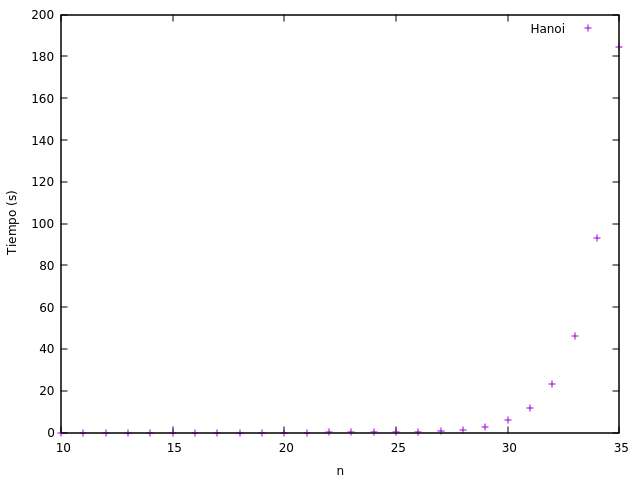
\includegraphics[width=95mm]{graficos/o2n}}
    \end{figure}
  
  \end{frame}

\subsection{Algoritmos de ordenaci�n}
\begin{frame}\frametitle{Algoritmos de ordenaci�n}

  \begin{figure}[H]
    \centering
    \subfigure{\label{graf:sort}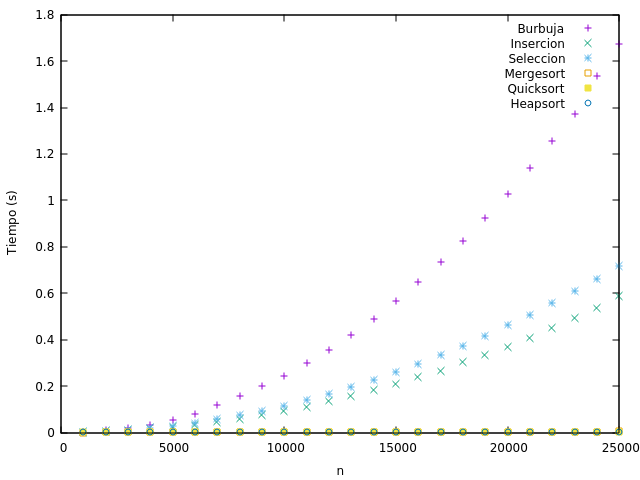
\includegraphics[width=95mm]{graficos/sort}}
    \end{figure}
  
\end{frame}

\section{Eficiencia H�brida}

\subsection{Algoritmos con orden de eficiencia $O(n^2)$}

\begin{frame}[fragile]\frametitle{Algoritmos con orden de eficiencia $O(n^2)$} 

\begin{equation*}
    f(x)=a_0x^2+a_1x+a_2
\end{equation*}

\vfill

\begin{flushleft}
  Coeficientes obtenidos para algoritmo de ordenaci�n por burbuja:
\end{flushleft}

\begin{verbatim}
Final set of parameters            Asymptotic Standard Error
=======================            ==========================
a0              = 2.87309e-09      +/- 3.994e-11    (1.39%)
a1              = -6.33841e-06     +/- 1.07e-06     (16.88%)
a2              = 0.014873         +/- 0.006036     (40.59%)
\end{verbatim}

\end{frame}

\begin{frame}\frametitle{Burbuja}

  \begin{figure}[H] \centering
\subfigure{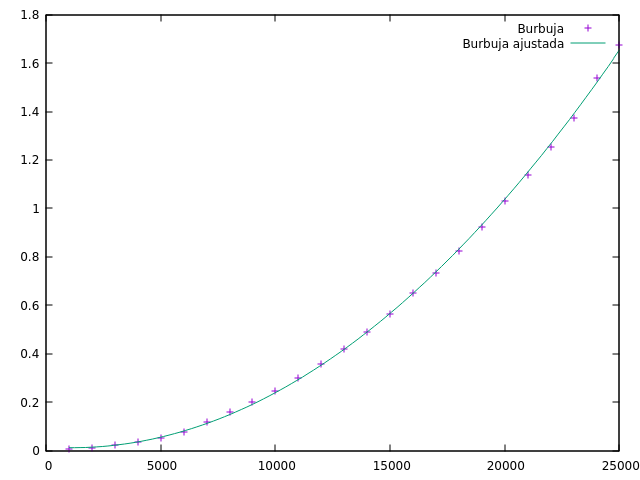
\includegraphics[width=95mm]{graficos/burbuja_ajust}}
\end{figure}

\end{frame}

\begin{frame}[fragile]\frametitle{Inserci�n}
  
\begin{verbatim}
Final set of parameters            Asymptotic Standard Error
=======================            ==========================
a0              = 9.49226e-10      +/- 8.518e-12    (0.8974%)
a1              = -5.93381e-07     +/- 2.282e-07    (38.45%)
a2              = 0.0039437        +/- 0.001287     (32.64%)
\end{verbatim}
\vspace{-3mm}
\begin{figure}[H] \centering
\subfigure{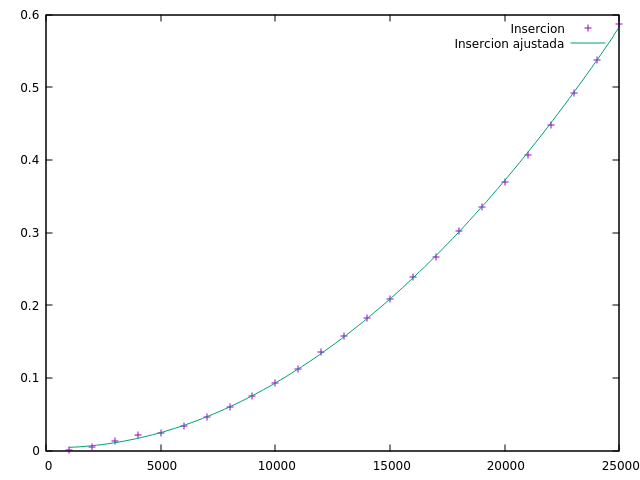
\includegraphics[width=70mm]{graficos/insercion_ajust}}
\end{figure}

\end{frame}

\begin{frame}[fragile]\frametitle{Selecci�n}
  
\begin{verbatim}
Final set of parameters            Asymptotic Standard Error
=======================            ==========================
a0              = 1.14435e-09      +/- 1.562e-12    (0.1365%)
a1              = 1.72508e-07      +/- 4.185e-08    (24.26%)
a2              = -0.000123672     +/- 0.0002361    (190.9%)
\end{verbatim}
\vspace{-3mm}
\begin{figure}[H] \centering
\subfigure{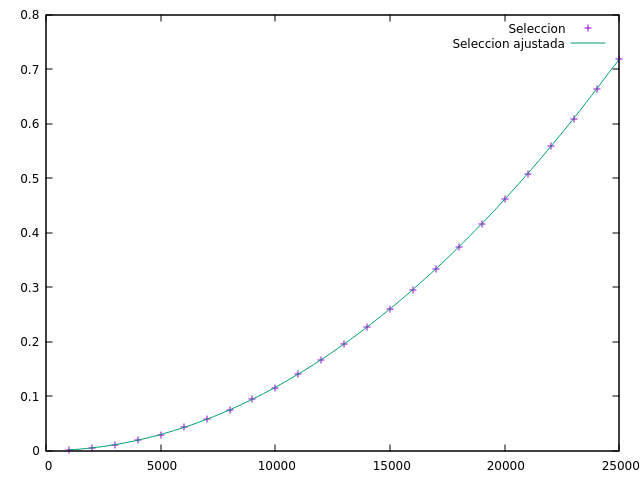
\includegraphics[width=70mm]{graficos/seleccion_ajust}}
\end{figure}

\end{frame}

\subsection{Algoritmos con orden de eficiencia $O(n\log n)$}

\begin{frame}[fragile]\frametitle{Algoritmos con orden de eficiencia $O(n\log n)$} 

\begin{equation*}
    f(x)=ax\log(bx+c)+d
\end{equation*}

\vfill

\begin{flushleft}
  Coeficientes obtenidos para mergesort:
\end{flushleft}

\begin{verbatim}
Final set of parameters            Asymptotic Standard Error
=======================            ==========================
a               = 6.95655e-08      +/- 1.431e-08    (20.57%)
b               = 0.000491397      +/- 0.0002775    (56.47%)
c               = 7.18312e-07      +/- 9.373e+04    (1.305e+13%)
d               = 0.000312996      +/- 13.27        (4.239e+06%)
\end{verbatim}

\end{frame}

\begin{frame}\frametitle{Mergesort}

\begin{figure}[H] \centering
\subfigure{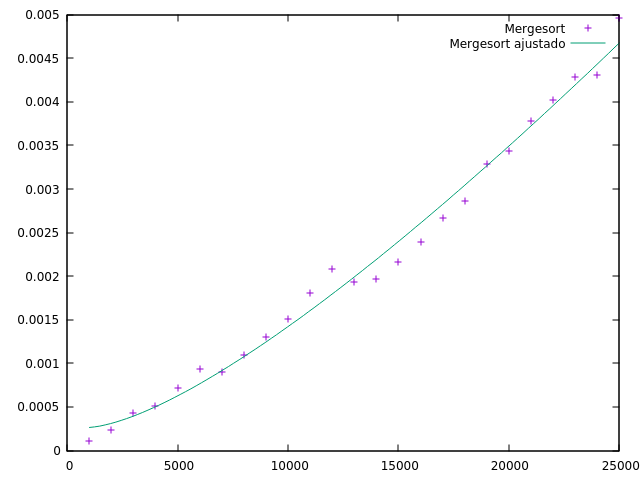
\includegraphics[width=95mm]{graficos/mergesort_ajust}}
\end{figure}

\end{frame}

\begin{frame}[fragile]\frametitle{Quicksort}
\vspace{-2mm}
\begin{verbatim}
Final set of parameters            Asymptotic Standard Error
=======================            ==========================
a               = 1.07312e-08      +/- 1.716e-08    (159.9%)
b               = 0.542892         +/- 8.438        (1554%)
c               = 7.18316e-07      +/- 2.12e+05     (2.951e+13%)
d               = 0.000390981      +/- 0.004212     (1077%)
\end{verbatim}
\vspace{-5mm}
\begin{figure}[H] \centering
\subfigure{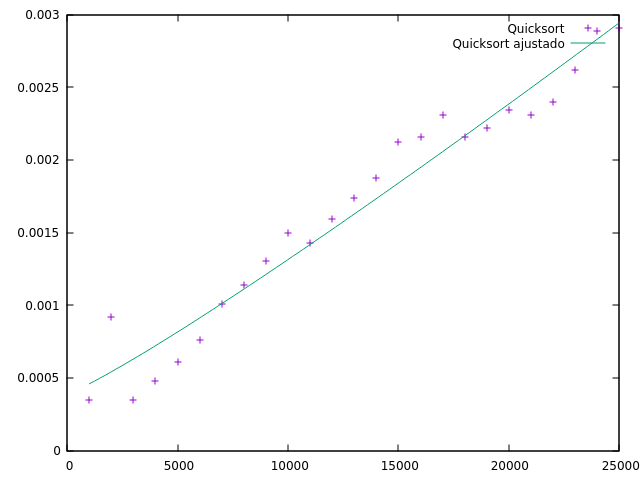
\includegraphics[width=70mm]{graficos/quicksort_ajust}}
\end{figure}

\end{frame}

\begin{frame}[fragile]\frametitle{Heapsort}
\vspace{-2mm}
\begin{verbatim}
Final set of parameters            Asymptotic Standard Error
=======================            ==========================
a               = 2.02343e-08      +/- 2.677e-08    (132.3%)
b               = -0.0611422       +/- 0.6122       (1001%)
c               = 2.74491e-06      +/- 7.44e+05     (2.711e+13%)
d               = 0.000535336      +/- 0.2463       (4.6e+04%)
\end{verbatim}
\vspace{-5mm}
\begin{figure}[H] \centering
\subfigure{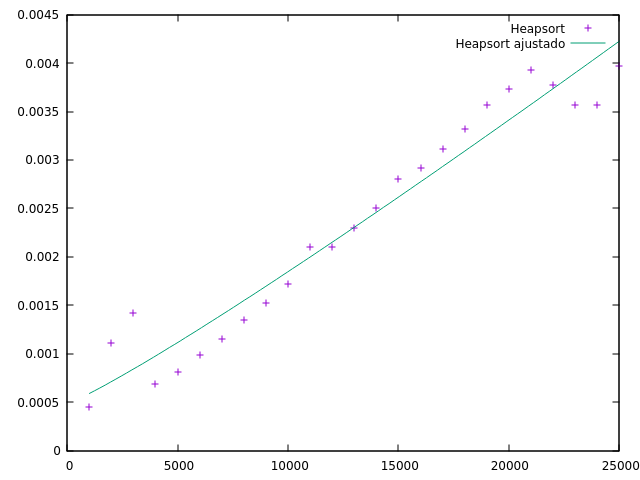
\includegraphics[width=70mm]{graficos/heapsort_ajust}}
\end{figure}

\end{frame}

\subsection{Algoritmos con orden de eficiencia $O(n^3)$: Algoritmo de Floyd}

\begin{frame}[fragile]\frametitle{Algoritmos con orden de eficiencia $O(n^3)$: Algoritmo de Floyd} 

\begin{equation*}
    f(x)=a_0x^3+a_1x^2+a_2x+a_3
\end{equation*}

\vfill

\begin{flushleft}
  Coeficientes obtenidos:
\end{flushleft}

\begin{verbatim}
Final set of parameters            Asymptotic Standard Error
=======================            ==========================
a0              = 4.6365e-09       +/- 1.322e-10    (2.851%)
a1              = 5.80584e-07      +/- 5.222e-07    (89.94%)
a2              = -0.00053539      +/- 0.0005904    (110.3%)
a3              = 0.111407         +/- 0.1808       (162.3%)
\end{verbatim}

\end{frame}

\begin{frame}

\begin{figure}[H] \centering
\subfigure{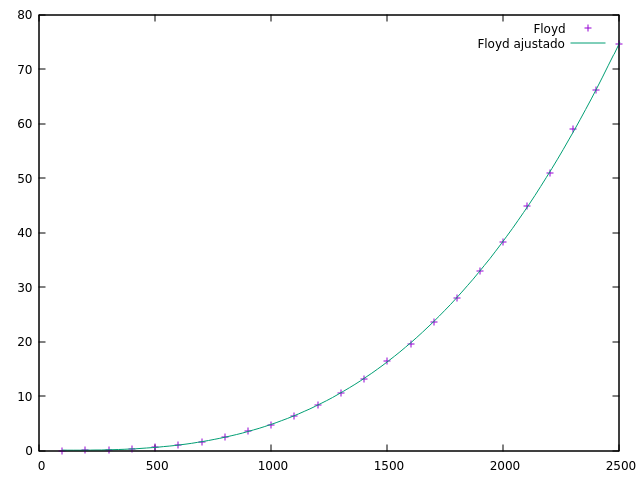
\includegraphics[width=95mm]{graficos/floyd_ajust}}
\end{figure}

\end{frame}

\subsection{Algoritmos con orden de eficiencia $O(2^n)$: Algoritmo de Hanoi}

\begin{frame}[fragile]\frametitle{Algoritmos con orden de eficiencia $O(2^n)$: Algoritmo de Hanoi} 

\begin{equation*}
    f(x)=a2^x+b
\end{equation*}

\vfill

\begin{flushleft}
  Coeficientes obtenidos:
\end{flushleft}

\begin{verbatim}
Final set of parameters            Asymptotic Standard Error
=======================            ==========================
a               = 5.33528e-09      +/- 2.615e-11    (0.49%)
b               = 1                +/- 0.2034       (20.34%)
\end{verbatim}

\end{frame}

\begin{frame}

\begin{figure}[H] \centering
\subfigure{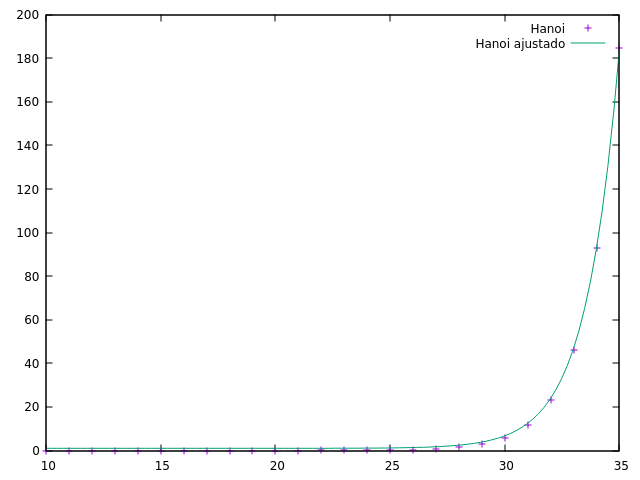
\includegraphics[width=95mm]{graficos/hanoi_ajust}}
\end{figure}

\end{frame}

\subsection{Otros ajustes}
\subsubsection{Mergesort}

\begin{frame}[fragile]\frametitle{Mergesort}

  \begin{equation*}
    f(x)=a_0x\log(a_1x+a_2)+a_3
  \end{equation*}
  \begin{equation*}
    g(x)=b_0x+b_1
  \end{equation*}
  \begin{equation*}
    h(x)=c_0x^2+c_1x+c_2
  \end{equation*}
  \vfill
  \begin{flushleft}
    Coeficientes obtenidos para $f$:
  \end{flushleft}
\begin{verbatim}
final sum of squares of residuals : 3.97491e-07

Final set of parameters            Asymptotic Standard Error
=======================            ==========================
a0              = 6.33118e-06      +/- 0.0005677    (8967%)
a1              = 5.89658e-07      +/- 5.426e-05    (9203%)
a2              = 1.01512          +/- 1.361        (134.1%)
a3              = 0.00010443       +/- 0.0001293    (123.8%)
\end{verbatim}
  
\end{frame}

\begin{frame}[fragile]\frametitle{Mergesort}
  \begin{flushleft}
    Coeficientes obtenidos para $g$:
  \end{flushleft}
\begin{verbatim}
final sum of squares of residuals : 1.11231e-06

Final set of parameters            Asymptotic Standard Error
=======================            ==========================
b0              = 1.90043e-07      +/- 6.099e-09    (3.209%)
b1              = -0.000322459     +/- 9.067e-05    (28.12%)
\end{verbatim}
\vfill
  \begin{flushleft}
    Coeficientes obtenidos para $h$:
  \end{flushleft}
\begin{verbatim}
final sum of squares of residuals : 3.96375e-07

Final set of parameters            Asymptotic Standard Error
=======================            ==========================
c0              = 3.64724e-12      +/- 5.786e-13    (15.86%)
c1              = 9.52149e-08      +/- 1.55e-08     (16.28%)
c2              = 0.000104267      +/- 8.744e-05    (83.86%)
\end{verbatim}

\end{frame}

\begin{frame}\frametitle{Mergesort}
  \begin{figure}[H] \centering
\subfigure{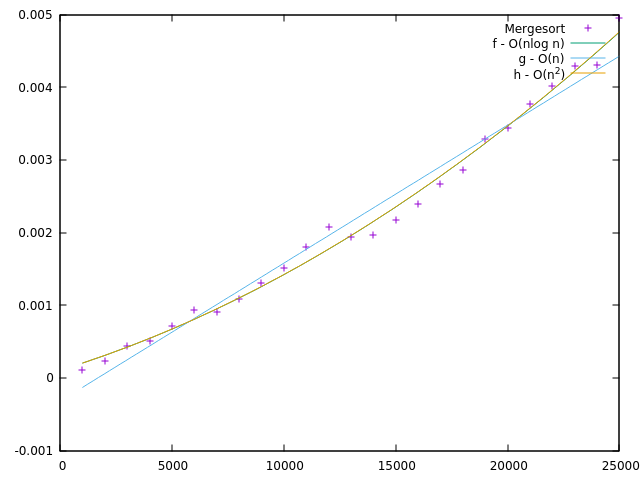
\includegraphics[width=95mm]{graficos/mergesort_otros_ajust}}
\end{figure}
\end{frame}

\subsubsection{Hanoi}

\begin{frame}[fragile]\frametitle{Hanoi}

  \begin{equation*}
    f(x)=a_02^x+a_1
  \end{equation*}
  \begin{equation*}
    g(x)=b_0x^{b_1}+b_2
  \end{equation*}
  \begin{equation*}
    h(x)=c_03^x+c_1
  \end{equation*}
  \vfill
  \begin{flushleft}
    Coeficientes obtenidos para $f$:
  \end{flushleft}
\begin{verbatim}
final sum of squares of residuals : 22.8446

Final set of parameters            Asymptotic Standard Error
=======================            ==========================
a0              = 5.33528e-09      +/- 2.615e-11    (0.49%)
a1              = 1                +/- 0.2034       (20.34%)
\end{verbatim}
  
\end{frame}

\begin{frame}[fragile]\frametitle{Hanoi}
  \begin{flushleft}
    Coeficientes obtenidos para $g$:
  \end{flushleft}
\begin{verbatim}
final sum of squares of residuals : 154.285

Final set of parameters            Asymptotic Standard Error
=======================            ==========================
b0              = 3.73043e-30      +/- 7.401e-30    (198.4%)
b1              = 20.5177          +/- 0.5393       (2.629%)
b2              = -1.27419         +/- 0.5837       (45.81%)
\end{verbatim}
\vfill
  \begin{flushleft}
    Coeficientes obtenidos para $h$:
  \end{flushleft}
\begin{verbatim}
final sum of squares of residuals : 1736.22

Final set of parameters            Asymptotic Standard Error
=======================            ==========================
c0              = 3.91192e-15      +/- 1.668e-16    (4.264%)
c1              = 1                +/- 1.736        (173.6%)
\end{verbatim}

\end{frame}

\begin{frame}\frametitle{Hanoi}
  \begin{figure}[H] \centering
\subfigure{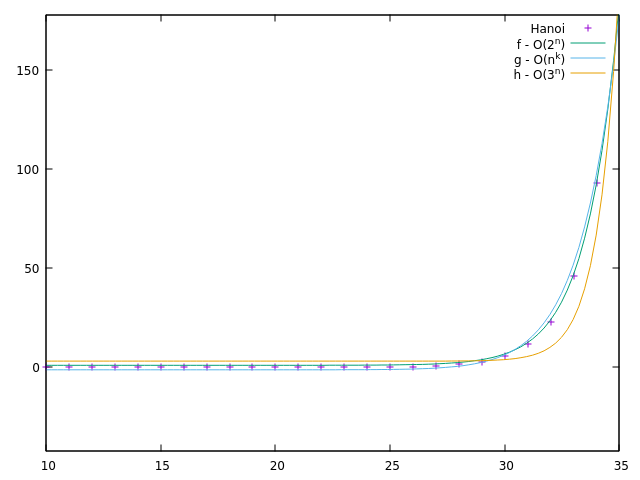
\includegraphics[width=95mm]{graficos/hanoi_otros_ajust}}
\end{figure}
\end{frame}

\section{Variaci�n de la eficiencia emp�rica con par�metros externos: Nivel de optimizaci�n}

\begin{frame}\frametitle{Burbuja}
  \begin{figure}[H] \centering
  \subfigure{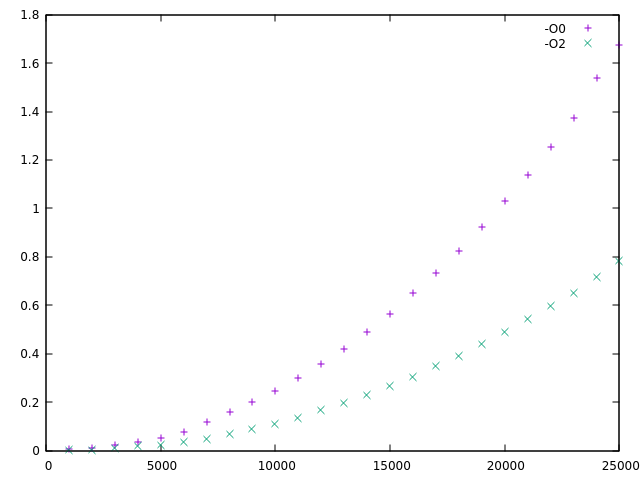
\includegraphics[width=95mm]{graficos/burbuja_op}}
\end{figure}
\end{frame}

\begin{frame}\frametitle{Quicksort}
  \begin{figure}[H] \centering
  \subfigure{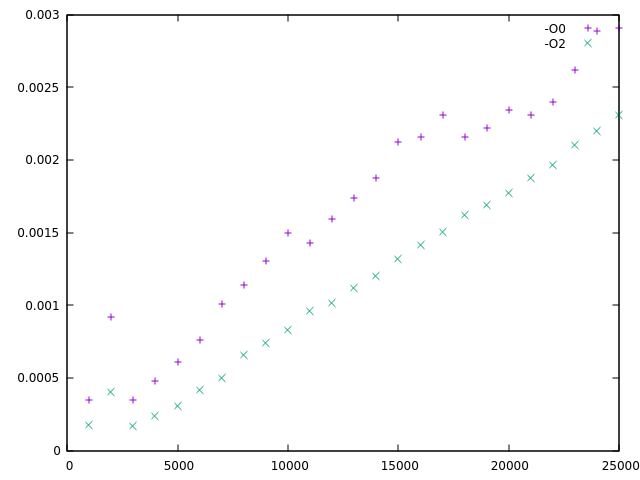
\includegraphics[width=95mm]{graficos/quicksort_op}}
\end{figure}
\end{frame}

\begin{frame}\frametitle{Floyd}
  \begin{figure}[H] \centering
  \subfigure{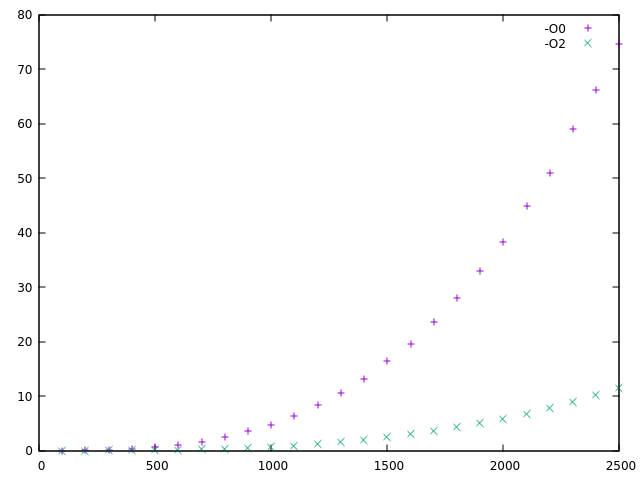
\includegraphics[width=95mm]{graficos/floyd_op}}
\end{figure}
\end{frame}

\begin{frame}\frametitle{Hanoi}
  \begin{figure}[H] \centering
  \subfigure{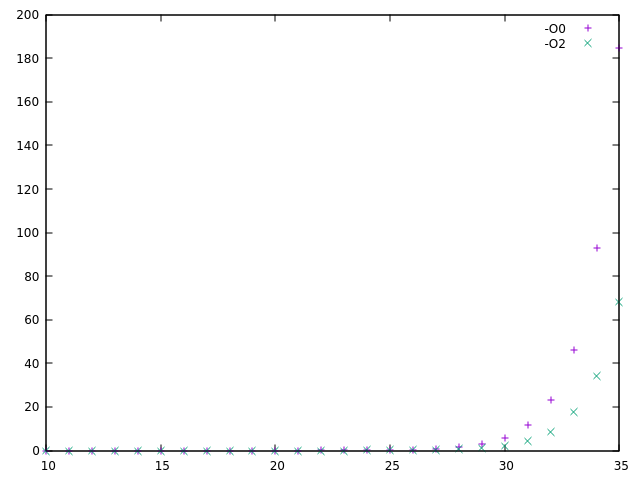
\includegraphics[width=95mm]{graficos/hanoi_op}}
\end{figure}
\end{frame}

\end{document}